\section{Auswertung}
\label{sec:Auswertung}
\subsection{Ausgangssignal}
\begin{figure}[H]
  \centering
  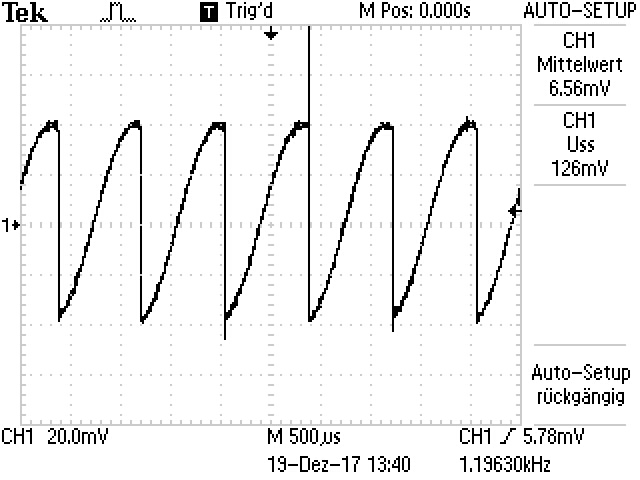
\includegraphics{content/images/0Phase.png}
  \caption{Ausgangssignal für \SI{0}{\degree} Phasenverschiebung.}
  \label{pic:0p}
\end{figure}
\begin{figure}[H]
  \centering
  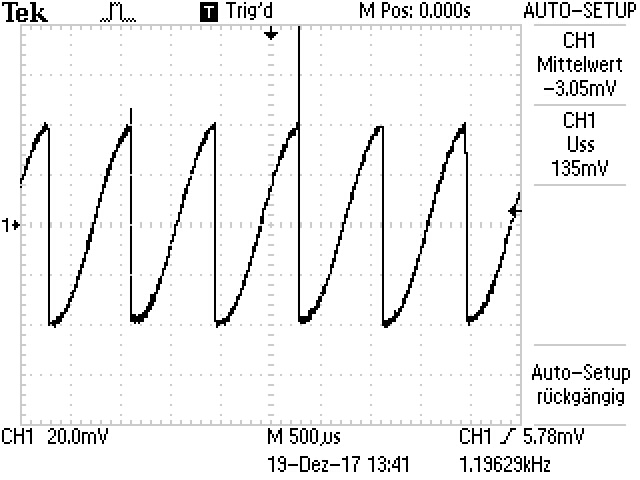
\includegraphics{content/images/30Phase.png}
  \caption{Ausgangssignal für \SI{30}{\degree} Phasenverschiebung.}
  \label{pic:3p}
\end{figure}
\begin{figure}[H]
  \centering
  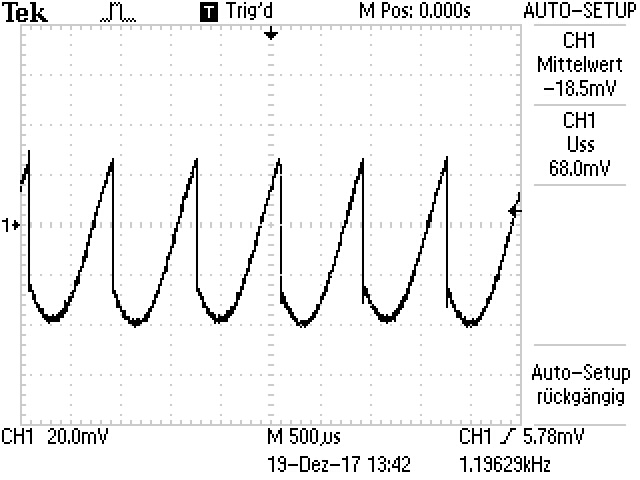
\includegraphics{content/images/60Phase.png}
  \caption{Ausgangssignal für \SI{60}{\degree} Phasenverschiebung.}
  \label{pic:6p}
\end{figure}
\begin{figure}[H]
  \centering
  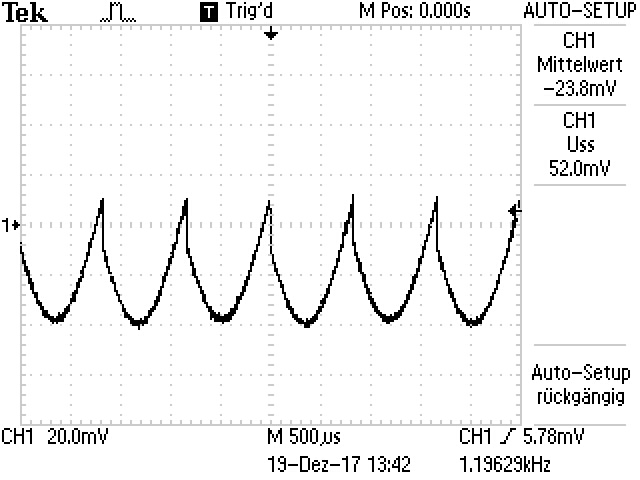
\includegraphics{content/images/90Phase.png}
  \caption{Ausgangssignal für \SI{90}{\degree} Phasenverschiebung.}
  \label{pic:9p}
\end{figure}
\begin{figure}[H]
  \centering
  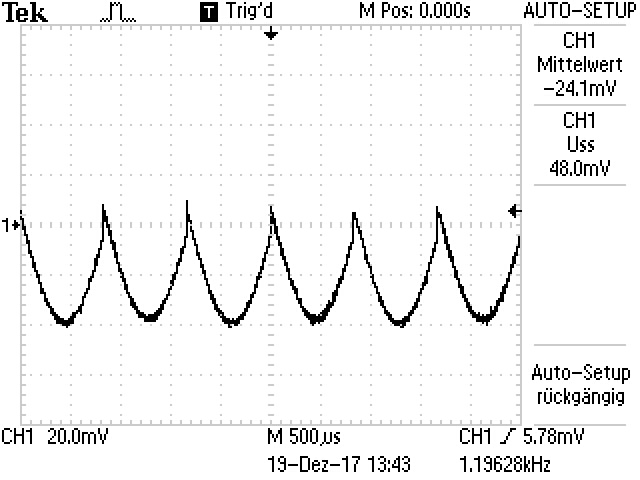
\includegraphics{content/images/120Phase.png}
  \caption{Ausgangssignal für \SI{120}{\degree} Phasenverschiebung.}
  \label{pic:12p}
\end{figure}
\subsection{Signalstärke in Abhängigkeit der Phase}

\begin{table}[H]
  \centering
  \caption{Phasenabhängigkeit mit und ohne Störsignal}
  \label{tab:data1}
  \sisetup{table-format=2.1}
  \begin{tabular}{S[table-format=3.0] S S}
    \toprule
    {$\text{Phase}$}&{$U_\text{out}\text{ ohne Störung}$}&{$U_\text{out}\text{ mit Störung}$} \\
    {$/\text{grad}$}&{$/V$}&{$/V$} \\
    \midrule
    0 &   6.6 &   5.6 \\
   15 &   2.2 &   2.8 \\
   30 &  -3.8 &  -4.2 \\
   45 & -14   & -11.6 \\
   60 & -18   & -19   \\
   75 & -22   & -22.5 \\
   90 & -25   & -24.5 \\
  105 & -23.6 & -25   \\
  120 & -20.8 & -24.5 \\
  135 & -17.6 & -22.5 \\
    \bottomrule
  \end{tabular}
\end{table}
[H]

\begin{figure}[H]
  \centering
  \includegraphics{build/phasen.pdf}
  \caption{Änderung der Phase ohne Störung.}
  \label{fig:ohne}
\end{figure}
\begin{figure}[H]
  \centering
  \includegraphics{build/phasen_mit.pdf}
  \caption{Änderung der Phase mit Störung.}
  \label{fig:mit}
\end{figure}

Regressionsgraphen der Form
\begin{equation}
  U(x)=a\text{cos}(\phi + b)
\end{equation}
Für die Messung ohne Störung ergibt sich:
\begin{gather*}
  a=\SI{23.68(94)}{\volt}\\
  b=\SI{1.32(4)}{}
  \intertext{unter Berücksichtigung des Gain x2000}
  a=\SI{11.84(47)e-3}{\volt}
\end{gather*}
Für die Messung mit Störung ergibt sich:
\begin{gather*}
  a=\SI{25.53(58)}{\volt}\\
  b=\SI{1.27(2)}{}
  \intertext{unter Berücksichtigung des Gain x2000}
  a=\SI{12.77(29)e-3}{\volt}
\end{gather*}
\subsection{Intensität der Diode}

\begin{table}[H]
  \centering
  \caption{Abstandserkennung}
  \label{tab:data2}
  \sisetup{table-format=2.1}
  \begin{tabular}{S S[table-format=1.2]}
    \toprule
    {$r$}&{$U_\text{out}$} \\
    {$/m$}&{$/V$} \\
    \midrule
    2.5 & 7.5  \\
    3.5 & 7    \\
    4.5 & 6.5  \\
    5.5 & 5.6  \\
    6.5 & 4.5  \\
    7.5 & 3.9  \\
    8.5 & 3.3  \\
    9.5 & 2.6  \\
   10.5 & 2.2  \\
   11.5 & 2    \\
   12.5 & 1.6  \\
   13.5 & 1.4  \\
   14.5 & 1.2  \\
   15.5 & 1.1  \\
   16.5 & 1    \\
   17.5 & 0.8  \\
   18.5 & 0.7  \\
   19.5 & 0.6  \\
   20.5 & 0.6  \\
   21.5 & 0.55 \\
   22.5 & 0.5  \\
   23.5 & 0.5  \\
   24.5 & 0.45 \\
   25.5 & 0.45 \\
   26.5 & 0.4  \\
   27.5 & 0.35 \\
   28.5 & 0.35 \\
   29.5 & 0.3  \\
   30.5 & 0.3  \\
   31.5 & 0.27 \\
    \bottomrule
  \end{tabular}
\end{table}
[H]
\begin{figure}[H]
  \centering
  \includegraphics{build/diode.pdf}
  \caption{Lichtintensität beim Abstand r.}
  \label{fig:diode}
\end{figure}

Regressionsgraph der Form
\begin{equation}
  U(x)=\frac{a}{r^2}
\end{equation}
Es ergibt sich:
\begin{gather*}
  a=\SI{24.54(24)e-3}{\volt}
  \intertext{unter Berücksichtigung des Gain x40}
  a=\SI{0.613(6)e-3}{\volt}
\end{gather*}
